% !TeX program = lualatex
% GitHub-facing variant of anc/TikZ/FusionScale4D.tex used as the README graphical abstract.
% The embedded space plane art and its annotation arrow are omitted here.
\documentclass[tikz,border=2pt]{standalone}

\usepackage{pgfplots,amsmath}
\pgfplotsset{compat=1.18}
\usetikzlibrary{shapes.geometric}
\usepgfplotslibrary{fillbetween}
\usepackage[colorlinks=true,linkcolor=blue,urlcolor=blue]{hyperref}

\begin{document}


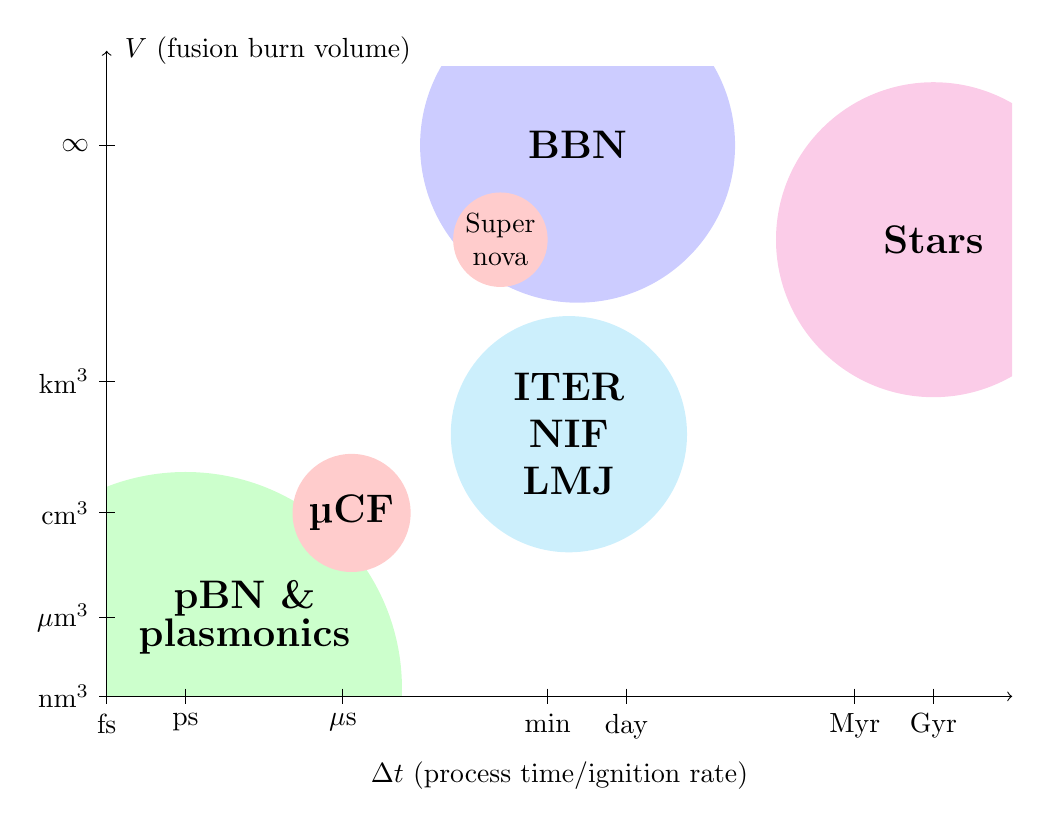
\begin{tikzpicture}[scale=1.0, transform shape]
%%%%%%%%%%
% Bubbles (background)
%%%%%%%%%%
\begin{scope}
\clip (0,0) rectangle (11.5,8);
% pB / plasmonics (nm-µm, fs-ps)
\fill[green!20] (1.0,0.10) circle[radius=2.75];
% μ-catalysed fusion (cm^3, µs)
\fill[red!20]  (3.11,2.33) circle[radius=0.75];
% NIF / LMJ (mm^3, ns)
%\fill[red!20]  (2.33,2.0)  circle[radius=0.60];
% Sandia Z Machine (cm^3, ~100 ns)
%\fill[red!20]  (2.67, 2.56)  circle[radius=0.30];
% ITER (10^3 m^3, ~400 s)
\fill[cyan!20]  (5.87,3.33) circle[radius=1.50];
% IEC fusor (100 cm^3, ms-s)
%\fill[red!20] (5.0,2.60) circle[radius=0.50];
% BBN (cosmic, ~15 min) - blue fill + red NE-SW hash
\fill[blue!20] (5.98,7.0) circle[radius=2.0];
%\fill[
%    pattern = neHatchWide,
%    pattern color=red,
%] (5.98,7.0) circle[radius=1.0];
% Stellar cores (Myr-Gyr, 10^25 m^3)
\fill[magenta!20] (10.5,5.8)  circle[radius=2.0];
% Brown dwarfs (10 kyr-10 Myr, 10^23 m^3)
%\fill[blue!20] (9.5,5.56)  circle[radius=0.6];
% Stellar supernova (~10^25 m^3, ~1 s)
\fill[red!20] (5.0,5.8) circle[radius=0.60];
\end{scope}

%%%%%%%%%%
% Labels (foreground)
%%%%%%%%%%
\begin{scope}
\node[align=center,scale=1.0] at (1.75,1.0) {\Large\textbf{pBN \&}\\\Large\textbf{plasmonics}};
\node[align=center,scale=1.0] at (3.11,2.33) {\Large\textbf{\textmu CF}};
%\node[align=center,scale=1.0] at (2.33,2.00) {NIF\\LMJ};
%\node[align=center,scale=1.0] at (2.67, 2.56) {Z};
\node[align=center,scale=1.0] at (5.87,3.33) {\Large\textbf{ITER}\\[0.5em]\Large\textbf{NIF}\\[0.5em]\Large\textbf{LMJ}};
%\node[align=center,scale=0.9] at (5.0,2.60) {\normalsize{IEC}};
\node[align=center] at (10.5,5.8) {\Large\textbf{Stars}};
%\node[align=center] at (9.5,5.56) {\small{Brown}\\\small{Dwarfs}};
\node[align=center] at (5.0,5.8) {\normalsize{Super}\\\normalsize{nova}};
\node[align=center] at (5.98,7.0) {\Large\textbf{BBN}};
\end{scope}

% Axes
\draw[->] (0,0) -- node[pos=0.5, below=20pt] {$\Delta t$ (process time/ignition rate)} (11.5,0);
\draw[->] (0,0) -- (0,8.2) node[above, right=3pt] {\(V\) (fusion burn volume)};

% x-axis ticks
\foreach \x/\lab in {
0/{fs},
1/{ps},
3/{\(\mu\)s},
5.6/{min},
6.6/{day},
9.5/{Myr},
10.5/{Gyr}
} {
\draw (\x,0.1)--(\x,-0.1) node[below] {\lab};
}

% y-axis ticks
\foreach \y/\lab in {
0/{\(\text{nm}^{3}\)},
1/{\(\mu\text{m}^{3}\)},
2.33/{\(\text{cm}^{3}\)},
4/{\(\text{km}^{3}\)},
%5.8/{stellar core},
7/{\(\infty\)}
} {
\draw (0.1,\y)--(-0.1,\y) node[left] {\lab};
}

\end{tikzpicture}

\end{document}
